\documentclass[tikz,border=3pt]{standalone}
\usepackage{pgfplots}\pgfplotsset{compat=1.18}
\usepackage{times}
\begin{document}
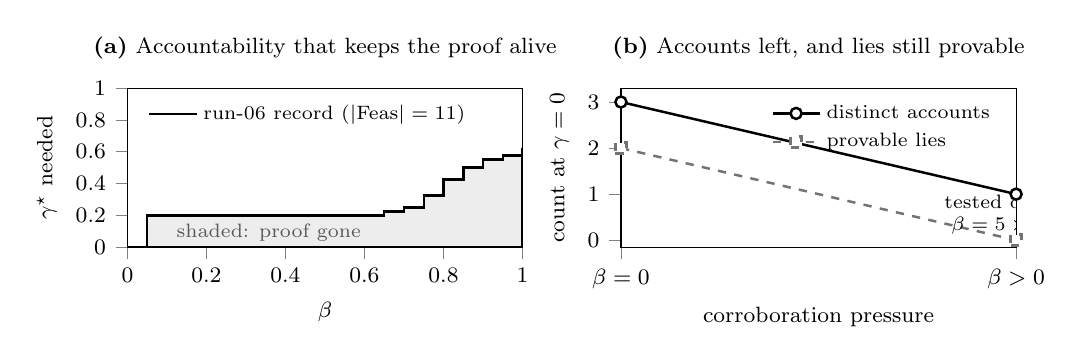
\begin{tikzpicture}
\pgfplotsset{
  every axis/.append style={font=\footnotesize, width=6.6cm, height=3.6cm,
    xmin=0, xmax=1, xlabel={$\beta$}, tick align=outside, tick pos=left,
    title style={font=\footnotesize, align=left, yshift=1pt},
    every axis plot/.append style={line width=0.9pt}},
}

%% ---- (a) the boundary ----
\begin{axis}[name=A, ymin=0, ymax=1,
  ylabel={$\gamma^\star$ needed},
  title={\textbf{(a)} Accountability that keeps the proof alive},
  legend style={font=\scriptsize, at={(0.03,0.97)}, anchor=north west, draw=none, fill=none},
  legend cell align=left]
\addplot[const plot, black, fill=black, fill opacity=0.07, draw opacity=1]
  coordinates {(0.000,0.000) (0.050,0.200) (0.100,0.200) (0.150,0.200) (0.200,0.200) (0.250,0.200) (0.300,0.200) (0.350,0.200) (0.400,0.200) (0.450,0.200) (0.500,0.200) (0.550,0.200) (0.600,0.200) (0.650,0.225) (0.700,0.250) (0.750,0.325) (0.800,0.425) (0.850,0.500) (0.900,0.550) (0.950,0.575) (1.000,0.625)} \closedcycle;
\addlegendentry{run-06 record ($|\mathrm{Feas}|=11$)}
\node[font=\scriptsize, text=black!65, anchor=west] at (axis cs:0.10,0.09)
  {shaded: proof gone};
\end{axis}

%% ---- (b) what collapses ---- placed to the RIGHT of (a), not below it:
%% stacked, this figure took a page of its own in a paper already over the limit.
\begin{axis}[name=B, at={(A.south east)}, anchor=south west, xshift=1.25cm,
  xmin=0, xmax=1, xtick={0,1},
  xticklabels={$\beta=0$,$\beta>0$}, xlabel={corroboration pressure},
  ymin=-0.15, ymax=3.3, ytick={0,1,2,3},
  ylabel={count at $\gamma=0$},
  title={\textbf{(b)} Accounts left, and lies still provable},
  legend style={font=\scriptsize, at={(0.97,0.97)}, anchor=north east, draw=none, fill=none},
  legend cell align=left]
\addplot[black, mark=*, mark options={fill=white}] coordinates {(0,3) (1,1)};
\addlegendentry{distinct accounts}
\addplot[black!55, dashed, mark=square*, mark options={fill=white}] coordinates {(0,2) (1,0)};
\addlegendentry{provable lies}
\node[font=\scriptsize, align=center, anchor=center] at (axis cs:1,0.55)
  {tested down to\\$\beta=5\times10^{-4}$};
\end{axis}
\end{tikzpicture}
\end{document}
